\documentclass[fleqn,11pt,openany]{book}

% These two need to be set before including scirun style package
\title{Transcranial Direct Current Stimulation Modeling Tutorial}
\author{Moritz Dannhauer}

% INCLUDE SCI STYLE DOCUMENT
\usepackage{scirun}
\usepackage{graphicx}
\usepackage{float}
\usepackage{hyperref}
\usepackage{subfigure}
% This makes displaying bold greek letters easier
\newcommand{\BM }[1]{\mbox{\boldmath $#1$}}

\begin{document}

%% starting from SCIRun Doc wiki


% CREATE TITLE PAGE --------------------------------------------------
\maketitle

% CHAPTERS ---------------------------------------------------------------

\chapter{Overview}

\begin{introduction}

This tutorial demonstrates how non-invasive electrical brain stimulation, known as transcranial direct current stimulation (tDCS), can be modelled using SCIRun.
It explains the basics of tDCS, the mathematical fundamentals, how to set up tDCS simulations as well as how to visualize results based on a simple geometric model: a label-mask data set containing multiple spheres forming a mickey mouse head).

\end{introduction}


\section{Transcranial Direct Current Stimulation (tDCS)}

Transcranial direct current stimulation (tDCS) is a non-invasive technique that effects human brain functions.
It is an emerging therapeutic approach to support the treatment of a wide range of neurological conditions, such as mood disorders, and is also known to enhance cognitive functions such as memory and motor skill learning.
tDCS is aiming to stimulate specific regions of the brain by injecting low amplitude direct currents through surface electrodes attached to the scalp of the subject.

\subsection{Mathematical Modeling}

For the purpose of computing a tDCS forward solution, the following equation system has to be solved: $M \cdot U = I$, where $M$ is the tDCS forward Matrix and $U$ is the solution potential vector given the injected current vector, the right hand side $I$.
$M$ combines volume conduction properties (FEM stiffness matrix) and electrical boundary conditions, including the complete electrode model to simulate current injection:

\begin{center}
\begin{eqnarray*}
     \nabla \cdot (\sigma \nabla u) & = & 0 ,(x \in \Omega), \\
     u + z_{l} \sigma \frac{\partial u}{\partial n} & = & 
     U_{l} , (on\ \partial \Omega_{e_{l}},x \in e_{l}),\\ 
     \int_{e_{l}} \sigma \frac{\partial u}{\partial n} & = & 
     I_{l} (l = 1,2,...,L), \\
      \sigma \frac{\partial u}{\partial n} & = & 
      0, (x \in \partial \Omega \setminus  \cup^{L}_{l=1} e_{l}). \\
\end{eqnarray*}
\end{center}

In more detail, $M$ is composed of the regular FEM stiffness ($A \in N \times N$, with $N$ representing the number of FEM nodes) and additional electrical boundary conditions specified as submatrices $A_{2}$,
$B$, $C$ ($B \in N \times L$, $C \in L \times L$, with $L$ representing the number of electrodes).
$M$ is composed such as: \\

\begin{eqnarray}
M &=& \left( \begin{array}{cc}
A & -B \\
-B^{T} & C
\end{array} \right) \nonumber \\
\left( \begin{array}{cc}
A & -B \\
-B^{T} & C
\end{array} \right) 
\left(
\begin{array}{c}
U_{n} \\
U_{e}
\end{array}
\right) &=& I =
\left(
\begin{array}{c}
I_{n} \\
I_{e}
\end{array}
\right) \nonumber, \\
A(i,j) &=& A_{1}(i,j) + A_{2}(i,j) = \int_{\Omega} \sigma \nabla \phi_{i} \cdot \nabla
\phi_{j}\ d\Omega + \nonumber \\
& & \sum_{l=1}^{L} \int_{e_{l}} \frac{1}{z_l} \phi_{i}
\phi_{j}\ d\Omega_{el}, \nonumber \\
B(i,l) &=& \frac{1}{z_{l}} \int_{e_l} \phi_{i}\ d\Omega_{el}
\nonumber, \\
C(i,l) &=& \frac{1}{z_{l}} \int_{e_l}\ d\Omega_{el}, \nonumber \\ \nonumber \\
\end{eqnarray}

Here, the donations are: $M \in \mathbb{R}^{N+L \times N+L}$, $A_{1},A_{2} \in \mathbb{R}^{N \times N}$, $B \in \mathbb{R}^{N \times L}$, $C \in \mathbb{R}^{L \times L}$, $U_n$ potentials at nodes, $U_e$ represents potentials at electrodes, $I_{e}$ is currents at electrodes and $\phi$ denotes linear basis functions. \\

The posed mixed electrical boundary problem can be efficiently solved with SCIRun modules (see more below).
The implemented complete electrode model enables to model a non-uniform current distribution across the surface of the electrodes. It also allows to 
adjust for the electrode-scalp contact relationship, using a resistive electrode impedance $z_{l}$, which is often available in experimental settings.

\chapter{Software requirements}

\section*{SCIRun Compability} 

The modules demonstrated in this tutorial are available in SCIRun version 4.7 and are not compatible with any older version of SCIRun.
Be sure to update your SCIRun version to the latest built available from the \href{http://www.scirun.org}{SCIRun website}, which will include the latest bug fixes and will make sure that the capabilities demonstrated in this tutorial are up to date.

\section*{Required Datasets} 

This tutorial relies on several datasets that are all part of the SCIRunData bundle.
To obtain these datasets, go to the \href{http://www.scirun.org}{SCIRun website} and click the \textbf{Download} button.
Instead of the SCIRun source or binary files, download the SCIRunData archive files.
The latter is available as a zip file or as a gzip file. 

\chapter{Finite Element Modeling}

We used a standard approach to solve finite element problems for tDCS (for details
\href{http://www.sci.utah.edu/devbuilds/scirun_docs/DefibrillationTutorial.pdf}{review the Defibrillation tutorial}, chapter 2).

\section{Preparation of Finite Element Model}

The finite element mesh (file name: mesh.mat) was generated using our meshing package
(\href{http://www.sci.utah.edu/cibc-software/cleaver-cibc.html}{cleaver}) based on the label mask file (file name: mickey4tDCS.nrrd).
The file mickey4tDCS.nrrd consists of the labels background, mickey's body, right ear, left ear and tDCS target region that have distinct label mask values 1, 2, 3, 4, 5.
The file mesh.mat (Matlab v6.0 format) contains a tetrahedra mesh with 54497 node locations defining 310856 tetrahedral elements.
Each of the tetrahedral elements is assigned to one of the five materials.

\section{Simulating Transcranial Direct Current Stimulation}\label{sec:sim_tdcs}

The SCIRun network used in this chapter can be found in the SCIRun nets directory in \\
\texttt{Optional/ElectricalBrainStimulation-Tutorial/SCIRUN\_TDCS\_simulation.srn}.

\subsection{Simulation Setting}

The simulation setup of the tDCS mickey mouse example contains 6 electrodes (depicted in red, see figure \ref{fig:sim_setting}) and one reference electrode 
(surface of mickey's right ear touching the head).
The target region is located deep (non-symmetrical in relation to center of the sphere) in mickey's head and is depicted in green in figure \ref{fig:sim_setting}.

\begin{figure}[!h]
\centering
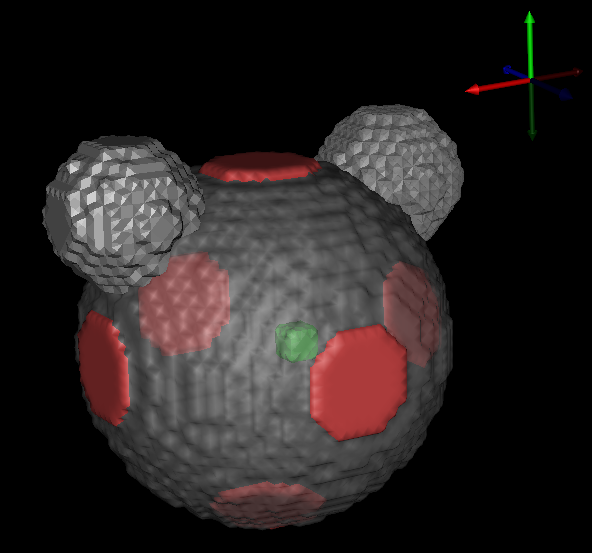
\includegraphics[width=0.5\textwidth]{ElectricalBrainStimulationTutorial_figures/sim_setting.png}
\caption{ tDCS simulation setting: mickey mouse toy example (coloring: red =electrodes, grey=mickey mouse body, green=tDCS target region)}
\label{fig:sim_setting}
\end{figure}

\subsection{Simulation Parameters}

There are three \href{http://scirundocwiki.sci.utah.edu/SCIRunDocs/index.php5/CIBC:Documentation:SCIRun:Reference:SCIRun:CreateMatrix}{CreateMatrix} modules in the upper part of SCIRun network \\
\texttt{SCIRUN\_TDCS\_simulation.srn} which are used to initiate simulation parameters.
The simulation domain only involves mickey's main body, which is essentially a single sphere (mickey's ears are removed), for a more efficient computational handling.
Note that, if simulations are based on SI units, with distances measured in meter ($m$), and mickey mouse body is over 10 m tall, amplitudes are given in Ampere $(A)$, electrical conductivities in Siemens/m $\left(\frac{S}{m}\right)$ and contact impedances are defined in Ohm/m $\left(\frac{\Omega}{m}\right)$.

\subsection{Setup Finite Element System}

The middle part of \texttt{SCIRUN\_TDCS\_simulation.srn} sets up and computes the tDCS forward solution (see figure \ref{fig:sim_femsetting}).
First, the stiffness matrix is computed using BuildFEMatrix module based on the tetrahedral mesh and conductivity information (taken from the CreateMatrix module labeled \textbf{CONDUCTIVITIES SIGMA}).
Second, the resulting stiffness matrix is piped into \href{http://scirundocwiki.sci.utah.edu/SCIRunDocs/index.php5/CIBC:Documentation:SCIRun:Reference:BioPSE:ApplyFEMVoltageSource}{ApplyFEMVoltageSource} module to set the first reference node of the mesh to be a constant zero potential to make the forward solution unique.
Third, the electrode parameters (electrode definition, figure \ref{fig:sim_setting} (contact impedances) were precomputed and loaded into SCIRun using a \href{http://scirundocwiki.sci.utah.edu/SCIRunDocs/index.php5/CIBC:Documentation:SCIRun:Reference:MatlabInterface:ImportMatricesFromMatlab}{ImportMatricesFromMatlab} module.
Fourth, the tDCS forward matrix $M$ is then piped into \href{http://scirundocwiki.sci.utah.edu/SCIRunDocs/index.php5/CIBC:Documentation:SCIRun:Reference:SCIRun:SolveLinearSystem}{SolveLinearSystem} and solved for the right hand side ($I_n$ = 0, $I_{e}\ \ne 0$ based on values from the CreateMatrix module labeled \textbf{AMPLITUDES}).
The result of SolveLinearSytem $U$ is reshaped to $U_{n}$ to match the number of nodes were its mapped onto in the next step.

\begin{figure}[!h]
\centering
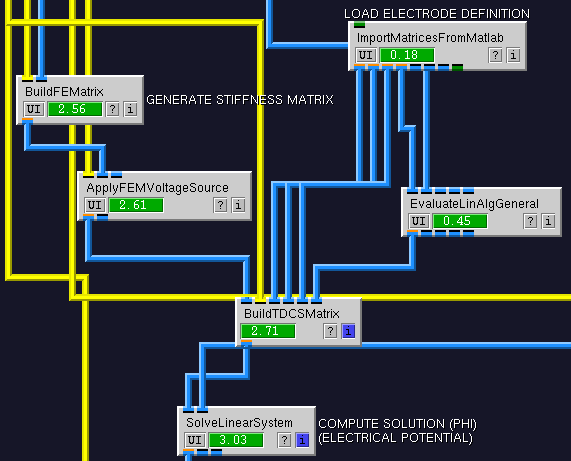
\includegraphics[width=0.8\textwidth]{ElectricalBrainStimulationTutorial_figures/fem_setup.png}
\caption{Setting up and computing tDCS forward solution.}
\label{fig:sim_femsetting}
\end{figure}

\subsection{Visualization of Results}

The visualization of tDCS results is located at the bottom of \\
\texttt{SCIRUN\_TDCS\_simulation.srn}.
The visualization results depend highly on simulation parameters.
For example, changing the electrical conductivity of the target region to a very small value (such as 0.00000001) will affect the current streamlines that will mainly flow around the tDCS target region.

\begin{figure}[!h]
\centering
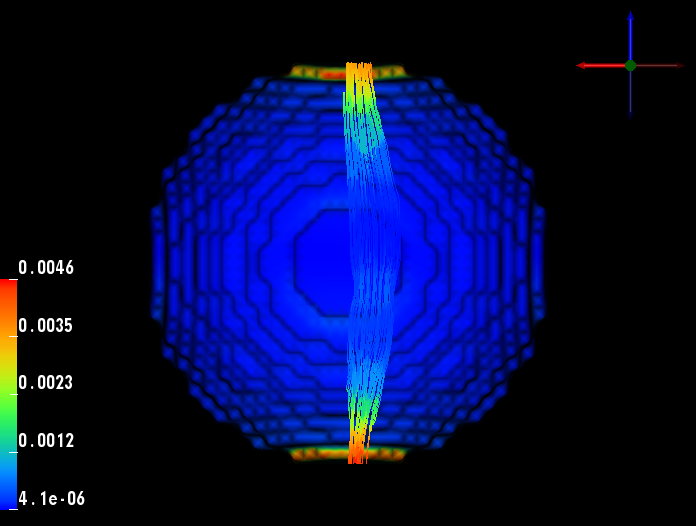
\includegraphics[scale=0.6]{ElectricalBrainStimulationTutorial_figures/current.png}
\caption{Visualization of tDCS simulation results: Electrical currents running through tDCS target region.}
\label{fig:sim_vis}
\end{figure}

\section{Optimization of Current Injection}

The electrical current optimization is based on the same finite element model as used in \autoref{sec:sim_tdcs} and can be found in the SCIRun nets directory in \\
\texttt{Optional/ElectricalBrainStimulation-Tutorial/SCIRUN\_TDCS\_optimization.srn}.

\subsection{Mathematical Modeling}

The optimization of injecting currents for a given ROI and current density (direction and magnitude) is performed in a minimum norm least square sense using a standard
SCIRun module called
\href{http://scirundocwiki.sci.utah.edu/SCIRunDocs/index.php5/CIBC:Documentation:SCIRun:Reference:BioPSE:SolveInverseProblemWithTikhonov}{SolveInverseProblemWithTikhonov}.
Therefore, an over-determined linear system has to be solved $\|  T \cdot I_{opt} - b \|$, where T is the transfer matrix ($T \in 3 \cdot M \times L$, $M$ being the number of finite elements, optimial current intensities $I_{opt}\ \in\ L\ \times\ 1$) and $b\ \in 3 \cdot M \times 1$ being the desired current density at the target ROI.
The transfer matrix T is composed of 6 columns ($L\ =\ 6$), each being a tDCS forward solution of a pair-wise current injection pattern (each electrode represents an anode and reference electrode being a cathode).

\subsection{Simulation Parameters}

In addition to \texttt{SCIRUN\_TDCS\_simulation.srn}, the Amplitude definition (since they are solved for) is removed and two more CreateMatrix Modules(\textbf{TARGET CURRENT DENSITY}, \textbf{TARGET CURRENT DIRECTION}) are added to the top part of \\
\texttt{SCIRUN\_TDCS\_optimization.srn} to control the optimization.

\subsection{Finite Element Setup and Optimization}

As mentioned above, the finite element problem has to be solved 6 times (once for each electrode) referentially regarding the reference electrode.
The optimization is based on the current density, meaning that, the gradient (for the 3 spatial directions: x, y and z) of the potential multiplied at each finite element by its
electrical conductivity needs to be computed.
The potential gradient is reshaped to fit a transfer matrix column $T$. The mesh elements of the target ROI are identified (precomputed) and the desired current density is assigned $b$.
$T$ and $b$ are piped into SolveInverseProblemWithTikhonov, a small regularization parameter is set and solved as an overdetermined problem for the 6 injected current intensities.  

\subsection{Visualization of Results}

As in \texttt{SCIRUN\_TDCS\_simulation.srn}, streamlines running through the ROI (\ref{fig:opt_sol}) are computed using \href{http://scirundocwiki.sci.utah.edu/SCIRunDocs/index.php5/CIBC:Documentation:SCIRun:Reference:SCIRun:GenerateStreamLines}{GenerateStreamLines} and electrical current density magnitude is mapped on them.
The optimized current intensities for the 6 electrodes can be reviewed in \href{http://scirundocwiki.sci.utah.edu/SCIRunDocs/index.php5/CIBC:Documentation:SCIRun:Reference:SCIRun:ReportStringInfo}{ReportStringInfo} module (bottom right part of the network).

\begin{figure}[!h]
\centering
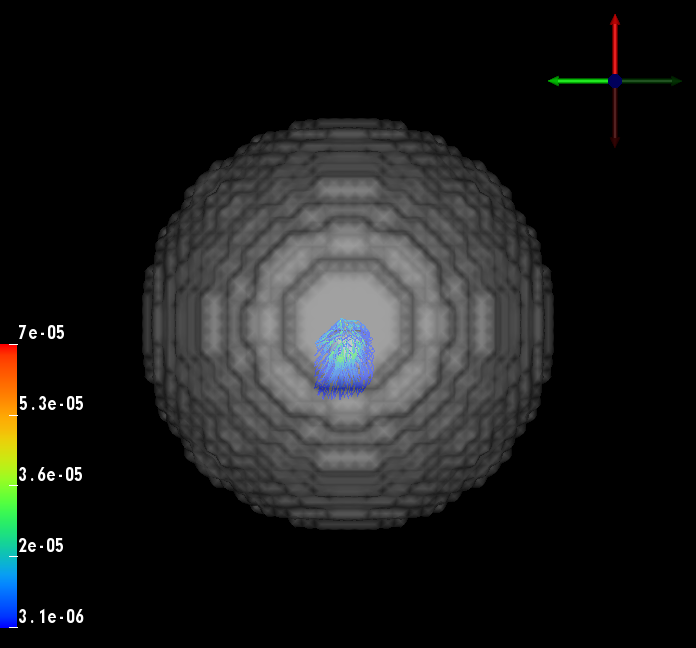
\includegraphics[width=0.6\textwidth]{ElectricalBrainStimulationTutorial_figures/opt_sol_downz.png}
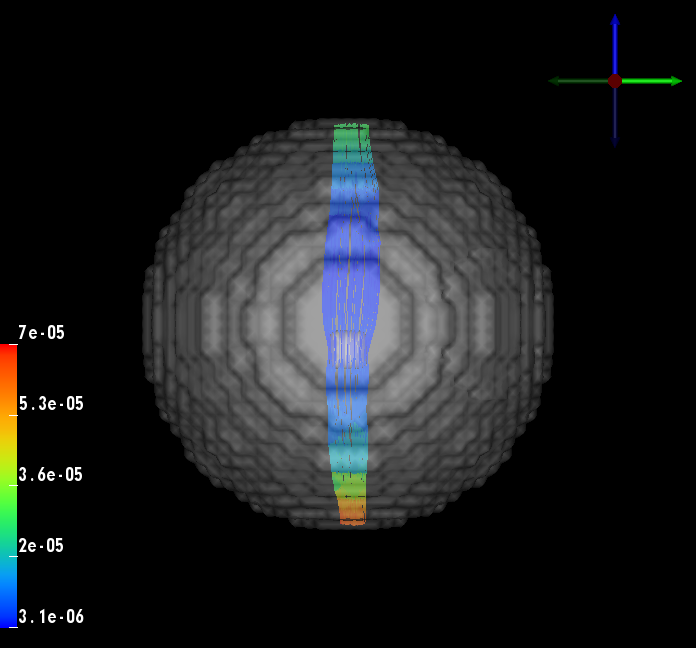
\includegraphics[width=0.6\textwidth]{ElectricalBrainStimulationTutorial_figures/opt_sol_downx.png}

\caption{Optimization result: Optimized current density streamlines depicts on x-y axis (top) and depicts x-z axis (bottom) (stimulated direction [0 0 1]) in ROI.}
\label{fig:opt_sol}
\end{figure}

\end{document}
